\documentclass[letterpaper,12pt,oneside]{book}

%%%%%%%%%%%%%%%%%%%%%%%%%%%%%%%%%%%%%%%%%%%%%%%%%%%%%%%%%%%%%%%
%%%%%%%%%%%%%%%%%%%%%%%%%%%%%%%%%%%%%%%%%%%%%%%%%%%%%%%%%%%%%%%
%                    Cosas para la portada                    %
%%%%%%%%%%%%%%%%%%%%%%%%%%%%%%%%%%%%%%%%%%%%%%%%%%%%%%%%%%%%%%%
%%%%%%%%%%%%%%%%%%%%%%%%%%%%%%%%%%%%%%%%%%%%%%%%%%%%%%%%%%%%%%%

\usepackage[dvipsnames]{xcolor}
\usepackage{tikz}
\usetikzlibrary{calc}
\usepackage{anyfontsize}
\usepackage{sectsty}


%%%%%%%%%%%%%%%%%%%%%%%%%%%%%%%%%%%%%%%%%%%%%%%%%%%%%%%%%%%%%%%
%%%%%%%%%%%%%%%%%%%%%%%%%%%%%%%%%%%%%%%%%%%%%%%%%%%%%%%%%%%%%%%

\usepackage[top=1in, left=1.25in, right=1.25in, bottom=1in]{geometry}

\usepackage{ 
comment,        %Para hacer comentarios largos
graphicx,       %Para meter figuritas
enumitem,       %Para hacer listas chidas (Paquete esencial en la vida)
amsfonts,       %Las letras de pizarra
amsmath,        %Fracciones, integrales y otras cosas
amsthm,         %Teoremas
amssymb,        %Más símbolos
mathtools,      %MÁS SÍMBOLOS
mathrsfs,       %Letras cursivas matemáticas
bm,             %Letras matemáticas negritas
bbm,            %Esta da la indicadora con \mathbbm 1
physics,        %Símbolos físicos
chronology,     %Líneas de tiempo
tikz            %Figuras
}
\usetikzlibrary{snakes}



\usepackage[ruled,vlined,spanish,onelanguage]{algorithm2e} %Algoritmos
\usepackage[utf8]{inputenc}
\usepackage[spanish,es-nodecimaldot]{babel} %Para que salgan las cosas en español

\pagestyle{empty}
\author{Pues yo, quién más\\[3pt]Editado por Inuzm \\[4pt] Queti}
\title{Finanzas para Cracks}

\begin{document}

\begin{tikzpicture}[overlay,remember picture]

% Background color
\fill[
black!2]
(current page.south west) rectangle (current page.north east);

% Rectangles
\shade[
left color=Dandelion, 
right color=Dandelion!40,
transform canvas ={rotate around ={45:($(current page.north west)+(0,-6)$)}}] 
($(current page.north west)+(0,-6)$) rectangle ++(9,1.5);

\shade[
left color=lightgray,
right color=lightgray!50,
rounded corners=0.75cm,
transform canvas ={rotate around ={45:($(current page.north west)+(.5,-10)$)}}]
($(current page.north west)+(0.5,-10)$) rectangle ++(15,1.5);

\shade[
left color=lightgray,
rounded corners=0.3cm,
transform canvas ={rotate around ={45:($(current page.north west)+(.5,-10)$)}}] ($(current page.north west)+(1.5,-9.55)$) rectangle ++(7,.6);

\shade[
left color=orange!80,
right color=orange!60,
rounded corners=0.4cm,
transform canvas ={rotate around ={45:($(current page.north)+(-1.5,-3)$)}}]
($(current page.north)+(-1.5,-3)$) rectangle ++(9,0.8);

\shade[
left color=red!80,
right color=red!80,
rounded corners=0.9cm,
transform canvas ={rotate around ={45:($(current page.north)+(-3,-8)$)}}] ($(current page.north)+(-3,-8)$) rectangle ++(15,1.8);

\shade[
left color=orange,
right color=Dandelion,
rounded corners=0.9cm,
transform canvas ={rotate around ={45:($(current page.north west)+(4,-15.5)$)}}]
($(current page.north west)+(4,-15.5)$) rectangle ++(30,1.8);

\shade[
left color=RoyalBlue,
right color=Emerald,
rounded corners=0.75cm,
transform canvas ={rotate around ={45:($(current page.north west)+(13,-10)$)}}]
($(current page.north west)+(13,-10)$) rectangle ++(15,1.5);

\shade[
left color=lightgray,
rounded corners=0.3cm,
transform canvas ={rotate around ={45:($(current page.north west)+(18,-8)$)}}]
($(current page.north west)+(18,-8)$) rectangle ++(15,0.6);

\shade[
left color=lightgray,
rounded corners=0.4cm,
transform canvas ={rotate around ={45:($(current page.north west)+(19,-5.65)$)}}]
($(current page.north west)+(19,-5.65)$) rectangle ++(15,0.8);

\shade[
left color=OrangeRed,
right color=red!80,
rounded corners=0.6cm,
transform canvas ={rotate around ={45:($(current page.north west)+(20,-9)$)}}] 
($(current page.north west)+(20,-9)$) rectangle ++(14,1.2);

% Year
\draw[ultra thick,gray]
($(current page.center)+(5,2)$) -- ++(0,-3cm) 
node[
midway,
left=0.25cm,
text width=5cm,
align=right,
black!75
]
{
{\fontsize{25}{30} \selectfont \bf Portada \\[10pt] Tikz}
} 
node[
midway,
right=0.25cm,
text width=6cm,
align=left,
orange]
{
{\fontsize{72}{86.4} \selectfont 2020}
};

% Title
\node[align=center] at ($(current page.center)+(0,-5)$) 
{
{\fontsize{60}{72} \selectfont {{Finanzas para Cracks}}} \\[1cm]
{\fontsize{16}{19.2} \selectfont \textcolor{orange}{ \bf Yo pues, quién más}}\\[3pt]
Editado por Inuzm\\[3pt]
Queti};
\end{tikzpicture}
\tableofcontents
\listoffigures

\chapter{Veamos algo de Tikz}

Tikz es una herramienta para crear gráficos en \LaTeX. 

\section{¿Por qué usar Tikz?}

Porque al usar comandos de dibujo, las imágenes no pierden calidad. Hay otros formatos para 

\begin{figure}[htp]
\centering
\begin{tikzpicture} % tikz environment   
  [scale=1,auto=center,every node/.style={circle,fill=red!10}] % here, node/.style is the style pre-defined, that will be the default layout of all the nodes. You can also create different forms for different nodes.  
    
  \node (a1) at (2.8844991406148166, 0) {$n_1$};  
  \node (a2) at (2.8844991406148166, 8)  {$n_2$};   
  \node (a3) at (0.0, 2)  {$n_3$};  
  \node (a4) at (5.768998281229633, 2) {$n_4$};  
  \node (a5) at (0.0, 6)  {$n_5$};  
  \node (a6) at (5.768998281229633, 6)  {$n_6$};  
  
  \draw (a1) -- (a2);
  \draw (a1) -- (a3);
  \draw (a1) -- (a4);
  \draw (a1) -- (a5);
  \draw (a1) -- (a6);
  \draw (a2) -- (a3);  
  \draw (a2) -- (a4);
  \draw (a2) -- (a5);
  \draw (a2) -- (a6);
  \draw (a3) -- (a4);
  \draw (a3) -- (a5);
  \draw (a3) -- (a6); 
  \draw (a4) -- (a5);  
  \draw (a4) -- (a6);
  \draw (a5) -- (a6);
\end{tikzpicture}
\caption{Mira qué chido se ve, hazle zoom we} 
\label{figCiu}
\end{figure}

\begin{figure}[htp]
\centering
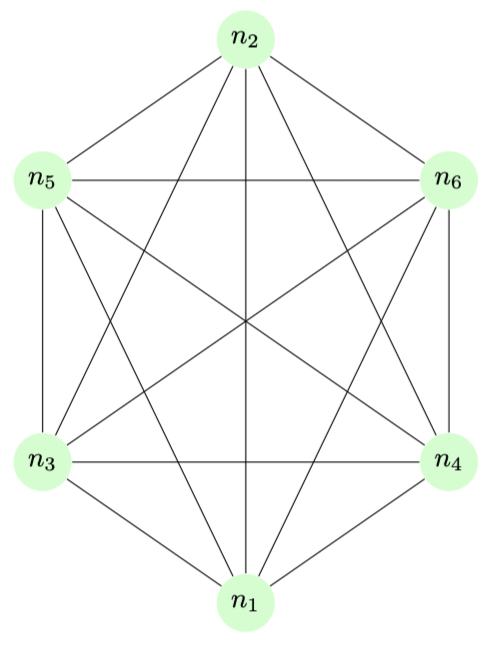
\includegraphics[width=5.5cm]{NoTikz}
\caption{Se ve fea, hazle zoom we} 
\label{fCF}
\end{figure}

Notemos que en la Figura \ref{figCiu} 

\section{Alternativas}
\begin{itemize}
\item Documentos \verb|.fig| de Matlab,
\item Documentos \verb|.ai| de Adobe Illustrator,
\item Imágenes en Power Point (no se recomienda).
\end{itemize}

\chapter{Líneas de tiempo}

\section{Los depósitos de David}
\noindent David desea realizar un depósito en una cuenta de ahorros. Esta cuenta de ahorros garantiza una tasa anual del 2 \% David va a depositar $\$300,000$ el día de hoy. Dentro de un año, David va a retirar la cantidad de $\$ 50,000$. Dentro de 3 años, depositará la cantidad de $\$500,000$. ¿Qué cantidad habrá en la cuenta dentro de 5 años? 

\begin{figure}[htp]
\centering
\begin{tikzpicture}
\draw (0,0) -- (5,0);
\foreach \x in {0, 1, 3, 5}
\draw (\x cm, 3pt) -- 	(\x cm, -3pt);
\draw (0,0) node[below = 3pt] {$0$};
\draw (0.5,0) node[above = 3pt]{\rotatebox{45}{$\$300,000$}};
\draw (1,0) node[below = 3pt] {$1$};
\draw (1.5,0) node[above = 3pt]{\rotatebox{45}{$-\$50,000$}};
\draw (3,0) node[below = 3pt] {$3$};
\draw (3.5,0) node[above = 3pt]{\rotatebox{45}{$\$500,000$}};
\draw (5,0) node[below = 3pt] {$5$};
\draw (5,0) node[above = 3pt]{\rotatebox{45}{$x$}};
\end{tikzpicture}	
\end{figure}

\begin{align*}
x &= 300,000 \cdot 1.02^{5}-50,000 \cdot 1.02^{4}+500,000 \cdot 1.02^{2}\\
  &= 797,302.633
\end{align*}

\noindent David tendrá $\$797,302.633$ dentro de 5 años en su cuenta de ahorros.\vspace{\baselineskip}

\noindent Luis Angel planea meter a su hijo de 10 años en la Ibero a la carrera de actuaría. Luis sabe que la colegiatura es de $\$240,000$ el año a la fecha de hoy. ¿Cuánto dinero pagará Luis para la carrera de su hijo si consideramos un interés del $6\,\%$? 

\begin{figure}[htp]
\centering
\begin{tikzpicture}
\draw (0,0) -- (1,0);
\draw[snake] (1,0) -- (3,0);
\draw (3,0) -- (7,0);

\foreach \x in {0, 4, 5, 6, 7}
\draw (\x cm, 3pt) -- 	(\x cm, -3pt);

\draw (0,0) node[below = 3pt] {$0$};
\draw (4,0) node[below = 3pt] {$8$};
\draw (5,0) node[below = 3pt] {$9$};
\draw (6,0) node[below = 3pt] {$10$};
\draw (7,0) node[below = 3pt] {$11$};

\draw (4.5,0) node[above = 3pt]{\rotatebox{45}{$\$240,000$}};
\draw (5.5,0) node[above = 3pt]{\rotatebox{45}{$\$240,000$}};
\draw (6.5,0) node[above = 3pt]{\rotatebox{45}{$\$240,000$}};
\draw (7.5,0) node[above = 3pt]{\rotatebox{45}{$\$240,000$}};
\end{tikzpicture}	
\end{figure}




\end{document}